\chapter{Dark solitons in BEC}
As a physical application of the code developed, we carried out simulations of the dynamics of a Bose-Einstein condensate (BEC). In particular we reproduced results of an experimental study performed at the National Institute of Standards and Technology (NIST), where they investigated the realization and evolution of solitons in a BEC of sodium atoms~\citep{DSF00}. In this chapter we briefly introduce the theoretical background of BEC and dark solitons, and proceed with the illustration of the simulation results, comparing them to the results of the NIST.

%%%%%%%%%%%%%%%%%%%%%%%%%%%%%%%%%%%%%%%%%%%%%%%%%%%%%%%%%%%%%%%%%%%%%%%%%%%%%%%%%%%%
\section{Theoretical background}
The dynamic of a weakly interacting Bose-Einstein condensate may be described by a non linear Schr\"odinger equation, namely the Gross-Pitaevskii equation~\citep{RC97,JKP98,DCLZ98,ZPMW99,DGPS99}.
%change these references
 Suppose we have a $N$-particle system, comprised of bosons interacting with each other. Using the Hartree approximation, we write the many-body wave function as
\begin{equation}
\psi(\textbf{r}_1, \textbf{r}_2,\ldots, \textbf{r}_N) = \prod_{i=1}^N \phi(\textbf{r}_i),
\end{equation}
where the single-particle wave function $\phi(\textbf{r}_i)$ is normalized in the usual way,
\begin{equation}
\int \mathrm{d}\textbf{r} \, |\psi(\textbf{r})|^2 = 1.
\end{equation} 
For low energy particles, the interaction can be described by an effective potential %(PS6.1)
that in coordinate space corresponds to a contact interaction $U_0 \delta(\textbf{r} - \textbf{r}')$, where $U_0 = 4 \pi \hbar^2 a_s / m$ and $a_s$ is the scattering length of the interaction~\citep{pethick2002bose}. Considering an external potential $V(\textbf{r}_i)$, the Hamiltonian may be written as
\begin{equation}
H = \sum_{i=1}^N \left[ \frac{\textbf{p}_i^2}{2 m} + V(\textbf{r}_i) \right] + U_0 \sum_{i<j} \delta(\textbf{r}_i - \textbf{r}_j).
\end{equation}
Then, the energy of the state is given by
\begin{equation}
E =  N \int \mathrm{d} \textbf{r} \, \left[ \frac{\hbar^2}{2m} |\nabla \phi(\textbf{r}) |^2 + V(\textbf{r}) |\phi(\textbf{r})|^2 + \frac{(N-1)}{2} U_0 |\phi(\textbf{r})|^4 \right].
\end{equation} 
It is convenient to introduce the concept of the wave function of the condensed state,
\begin{equation}
\psi(\textbf{r}) = N^{1/2} \phi(\textbf{r}),
\end{equation}
so that the normalization condition becomes
\begin{equation} \label{eq:normalization-N}
\int \mathrm{d}\textbf{r} \, |\psi(\textbf{r})|^2 = N.
\end{equation}
Moreover, we suppose that $N \gg 1$ so that the energy can be rewritten as,
\begin{equation}
E = \int \mathrm{d} \textbf{r} \, \varepsilon  = \int \mathrm{d} \textbf{r} \, \left[ \frac{\hbar^2}{2m} |\nabla \psi(\textbf{r}) |^2 + V(\textbf{r}) |\psi(\textbf{r})|^2 + \frac{1}{2} U_0 |\psi(\textbf{r})|^4 \right].
\end{equation}
The equation of motion may be derived from the principle of least action 
\begin{equation}
\delta \int_{t1}^{t2} \mathrm{d} t \, L = 0 \label{eq:least-principle}
\end{equation}
where the Lagrangian $L$ is given by
\begin{equation}
L = \int \mathrm{d} \textbf{r} \, \left[ \frac{\imath \hbar}{2} \left( \psi^\ast \frac{\partial \psi}{\partial t} - \psi \frac{\partial \psi^\ast}{\partial t} \right) - \varepsilon \right].
\end{equation}
Requiring that the variation of the independent variables $\psi(\textbf{r},t)$ and $\psi^\ast (\textbf{r},t)$ vanishes at $t=t_1$ and $t=t_2$, and on any spatial boundaries, from Eq.~\eqref{eq:least-principle} one finds the Gross-Pitaevskii equation:
\begin{equation} \label{eq:gross-pitaevskii}
\imath \hbar \frac{\partial \psi(\textbf{r}, t)}{\partial t} = \left[ - \frac{\hbar^2}{2m} \nabla^2 + V(\textbf{r}) + U_0 |\psi(\textbf{r}, t)|^2 \right] \psi(\textbf{r}, t).
\end{equation}

Formally, Eq.~\eqref{eq:gross-pitaevskii} is not implemented in our code since the Hamiltonian is not simply comprised of a kinetic term and an external potential term. However, if we denote $\tilde{V}(\textbf{r}, \psi(\textbf{r}, t)) = V(\textbf{r}) + U_0 |\psi(\textbf{r}, t)|^2$, the single time step evolution still has the form~\eqref{eq:single-iteration} and the exponential operator $\exp \left( - \frac{\imath}{\hbar} \tilde{V}(\textbf{r}, \psi(\textbf{r}, t)) \right)$ is still diagonal in the coordinate representation. Thus, we only have to define the potential such that, in the computational step 5 (Fig.~\ref{fig:scheme-iteration}), each site $(i,j)$ is also multiplied by the factor $\exp(-\frac{\imath}{\hbar} U_0 |\psi(i,j)|^2)$ where $\psi(i,j)$ is the wave function calculated in the previous computational step.

The ground-state of the system may be found numerically using the imaginary time evolution. However, for sufficiently large number of atoms an accurate expression is obtained using the Thomas-Fermi approximation. Suppose that the contribution of the kinetic energy term is negligible with respect to the one of the interaction term. Then the ground-state is approximated by the solution of the time independent Gross-Pitaevskii equation deprived of the kinetic term
\begin{equation}
\left[ V(\textbf{r}) + U_0 |\psi(\textbf{r})|^2 \right] \psi(\textbf{r}) = \mu_{TF} \psi(\textbf{r}),
\end{equation}
where $\mu$ is the chemical potential. This gives the solution
\begin{equation}
n(\textbf{r}) = |\psi(\textbf{r})|^2 = \frac{\mu_{TF} - V(\textbf{r})}{U_0},
\end{equation}
%check if I need to put abs in U_0
for $\textbf{r}$ such that $V(\textbf{r}) < \mu_{TF}$. 
For a BEC trapped in a harmonic potential of the form
\begin{equation}
V(x,y) = \frac{m}{2} (\omega_1^2 x^2 + \omega_2^2 y^2)
\end{equation}
the extension of the condensate wave function in the two directions is given by the two semi-axes
\begin{equation} \label{eq:TF-radius}
R_i = \sqrt{\frac{2\mu_{TF}}{m\omega_i^2}}, \, i = 1,2
\end{equation}
and the particles density has the form of an inverted parabola. Given the normalization condition in Eq.~\eqref{eq:normalization-N}, the chemical potential is determined as a function of $U_0$, and the system dimension (see Appendix~\ref{App:A}).

The Thomas-Fermi approximation gives an accurate description of the bulk properties of the system, but it fails near the edge of the cloud. Provided that $V(\textbf{r})$ varies slowly, a better solution for the ground state may be found solving the entire time independent Gross-Pitaevskii equation taking the linear term of the external potential at the edge of the cloud~\citep{pethick2002bose}.
%ref PS6.3

However, the Gross-Pitaevskii equation has exact analytical solutions in the nonlinear regime. These solutions have the form of solitary waves, called solitons, which are localized disturbances that propagate without changing of form. This phenomenon is due to the balance between dispersion and non linearity, which in Eq.~\eqref{eq:gross-pitaevskii} correspond to the kinetic term and the non linear interaction respectively. Solitons appear in different contexts of science and engineering, such as the dynamics of waves in shallow water~\citep{B88}, transport along DNA and other macromolecules~\citep{P95}, and fiber optic communications~\citep{H90}.
Depending on the details of the governing nonlinear equation, they can be either bright or dark. The former are peaks in the amplitude, while the latter are notches with a characteristic phase step across it. In the present work we focus on dark solitons. 

For BEC with repulsive interaction between the atoms, solitons present a depression in the density profile -- dark soliton. In a homogeneous BEC, the resulting density profile along the x axis is
\begin{equation}
n(x,t) = n_{min} + \left(n_0 - n_{min}\right)\tanh^2 \left( \frac{x - \nu_s t}{\sqrt{2} \xi} \sqrt{1 - \left( \frac{\nu_s}{\nu_0} \right)^2 } \right)
\end{equation}
where $n_0$ is the unperturbed density, $n_{min}$ is the density at the center of the soliton, $\nu_s$ and  $\nu_0 = (\frac{nU_0}{m})^{\frac{1}{2}}$ are the speed of the soliton and the speed of sound respectively, and 
\begin{equation}
\xi = \frac{\hbar}{\left( 2mn_0 U_0 \right)^{1/2}}
\end{equation}
being the healing length~\citep{pethick2002bose}.
%PS(7.6)
The speed and the depth of the soliton can be related with each other~\citep{RC97,JKP98}. Indeed, the soliton speed $\nu_s$ can be expressed as
\begin{equation} \label{eq:soliton-speed-density}
\nu_s = \nu_0 \sqrt{ \frac{n_{min}}{n} }.
\end{equation}
Note that the soliton speed is less than the speed of sound.
The soliton speed can also be expressed by means of the change in phase of the wave function across it:
\begin{equation}
\nu_s = \nu_0 \cos \left( \frac{\delta}{2} \right).
\end{equation}

Remarkably, the motion of a soliton in a BEC in an external potential is the same as that of a particle of mass $2m$ in the same potential~\citep{pethick2002bose}.
%ref PS(7.6) 
Consequently, for a potential having a minimum, the period of the motion of a soliton is $\sqrt{2}$ times that of a particle of mass $m$ in the potential.

%%%%%%%%%%%%%%%%%%%%%%%%%%%%%%%%%%%%%%%%%%%%%%%%%%%%%%%%%%%%%%%%%%%%%%%%%%%%%%%%%%%%%
\section{Soliton simulation}
In the experiments carried out in~\citep{DSF00}, the generation and propagation of solitons were studied in BEC of sodium atoms, confined in a magnetic trap. The magnetic trap generated a harmonic external potential with frequencies $\omega_x = \sqrt{2}\omega_y = 2 \omega_z = 2 \pi \cdot 28\,$Hz, while the system were composed by  $1.7 (\pm 0.3) \cdot 10^6$ atoms in the $3S_{1/2}$, $F=1$, $m_F=-1$ state\footnote{In this configuration the scattering length is $2.75$ nm~\citep{DSF00}.}. 

In this experiment, the system is three-dimensional, while our implementation is designed for a two-dimensional system. This would not be a problem if the dynamic of the 3D system was described by three decoupled equations, so that we could independently solve the two corresponding to the variables that span a 2D plane and ignore the other one. The Gross-Pitaevskii equation \eqref{eq:gross-pitaevskii} cannot be decoupled due to the non linear term, so this does not apply to our case. However, our purpose is to study the evolution of a soliton which propagates in one dimension, so we can ignore the dynamic along one of the two dimensions perpendicular to the axis of propagation. An approach to reduce to a two dimensional problem is to make a phenomenological hypothesis about the form of the solution. In the literature~\citep{JKP98,SZ98,Sal01,SPR02,MM03}, one can find several methods to reduce a 3D problem to a 2D one; we adopt the method described in~\citep{PietroMassignan}.
%non è un ipotesi avere la stessa dimensione, ma è lo scopo della procedura
 The hypothesis behind the method is that the solution of the reduced system has the same spatial extent of the original one. Since the 3D system is well described by the Thomas-Fermi approximation\footnote{The experimental configuration satisfies the conditions to adopt the Thomas-Fermi approximation.}, the extension of the ground state is known (Eq.~\eqref{eq:TF-radius}). Then, the approach is to rewrite the coupling constant $U_0^{(2)}$ for the 2D system, such that the chemical potential for the 2D system is the same as the one of the 3D system. This will ensure that the spatial extension of the 2D system will be the same as the 3D system (see Appendix~\ref{App:A}). For our simulation we reduced the dimension keeping the $x$ and $y$ axes of the 3D system. The resulting Gross-Pitaevskii equation for the 2D system becomes:
\begin{equation} \label{eq:gross-pitaevskii-simulation}
\imath \hbar \frac{\partial \psi(\textbf{r}, t)}{\partial t} = \left[ \sum_{i=1}^2 \left( -\frac{\hbar^2}{2m} \frac{\partial^2}{\partial x_i^2} + \frac{m}{2} \omega_i^2 x_i^2 \right) + U_0^{(2)} |\psi(\textbf{r}, t)|^2 \right] \psi(\textbf{r}, t),
\end{equation}
where
\begin{equation}
U_0^{(2)} = \frac{\pi}{2} \frac{\mu_{TF}}{N} \left( \bar{R}_{TF} \right)^2 ,
\end{equation}
with $\bar{R}_{TF} = \sqrt{2\mu_{TF} / m \bar{\omega}^2}$ the mean Thomas-Fermi radius, $\bar{\omega} = \sqrt{ \omega_x \omega_y}$ the geometric mean of the frequencies,
and $\mu_{TF}$ is the chemical potential in the Thomas-Fermi approximation for the 3D system
\begin{equation}
\mu_{TF} = \frac{1}{2} \left( 15 N \hbar^2 \omega_x \omega_y \omega_z \sqrt{m} a_s \right)^{2/5}
\end{equation}
\\

\noindent \textbf{Ground state.} According to the experiment, the BEC is initially described by the ground state  of Eq.~\eqref{eq:gross-pitaevskii}. They found it to have a spatial extension described by the Thomas-Fermi diameters of $2R_{TF, x} = 45 \, \mathrm{\mu m}$, $2R_{TF, y} = 64 \, \mathrm{\mu m}$ and $2R_{TF, z} = 90 \, \mathrm{\mu m}$, with a uniform phase~\citep{DGPS99}.
In the simulation, we approximated the ground state of Eq.~\eqref{eq:gross-pitaevskii-simulation} using imaginary time evolution. We proceed by taking a gaussian initial state, evolving it in imaginary time for a fixed number of iterations and then calculating the energy of the resulting state. Repeating this procedure using as initial state the one resulting from the last iteration, the energy decreases converging to the ground state energy. If we call $E_i$ the energy of the state resulting from the $i-$th iteration, we stopped the procedure once the $i-$th state satisfied the convergence condition
\begin{equation}
\left| \frac{E_{i} - E_{i-1}}{E_{i-1}} \right| < 10^{-6}.
\end{equation}
This ensure that the $i-$th state is an accurate approximation of the ground state. In Fig.~\ref{plot:density_x} and Fig.~\ref{plot:density_y} the profiles of the particle density along the two axes are shown. The particles density of the calculated ground state is in good agreement with the particles density of the Thomas-Fermi approximation and with the experimental results.
%put y instead x; try to put them side-by-side
\begin{figure}[t!]
   \centering
   \begin{tabular}{c}
      \subfloat[]{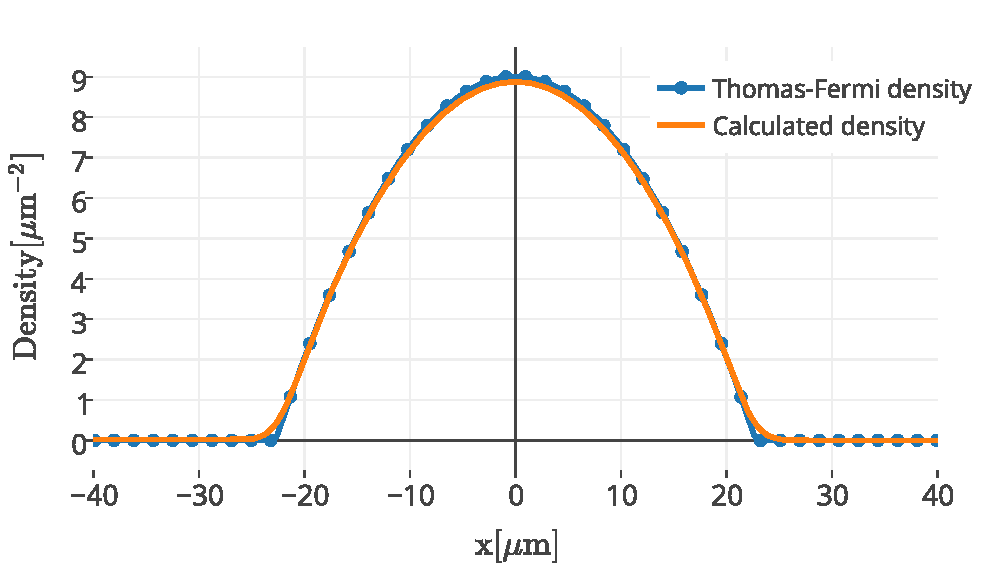
\includegraphics[width=8.5cm]{Plots/density_profile_x.pdf} \label{plot:density_x}}  \\
      \subfloat[]{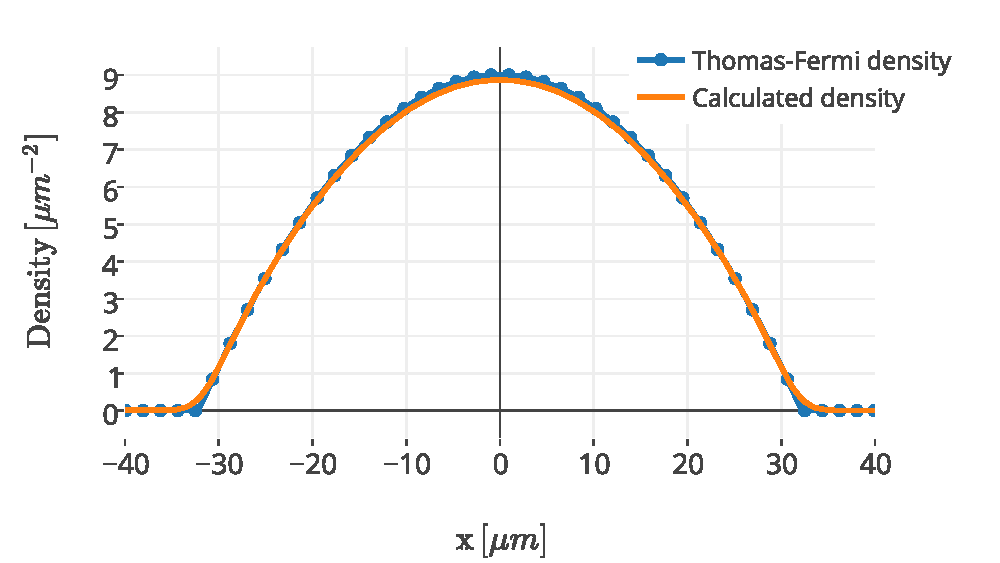
\includegraphics[width=8.5cm]{Plots/density_profile_y.pdf} \label{plot:density_y}} \\
   \end{tabular}
   \caption{Calculated ground-state density along the $x$ axis (a) and the $y$ axis (b). The simulation is in good agreement with the Thomas-Fermi approximation. The spatial extension of the  calculated ground state corresponds to the experimental results, where $R_{TF,x} =  45 \, \mathrm{\mu m}$ and $2R_{TF, y} = 64 \, \mathrm{\mu m}$.}
\end{figure}
\\

\noindent \textbf{Soliton propagation.} Solitons can be generated in BEC by phase imprinting. The phase of the ground state is modified by exposing the cloud to pulsed, off-resonant laser light with an intensity pattern $I(x,y)$. The wave function acquires a corresponding phase $\phi(x,y)$ proportional to $I(x,y)$ and the time of exposure $T$. According to the experiment, they chose $T$ to be short enough so that the atomic motion was negligible (Raman-Nath regime). In this condition, the effect of the pulse can be expressed as a sudden phase imprint, $\psi \rightarrow \psi \exp(\imath \phi(x,y))$~\citep{DSF00}. If the center of the BEC correspond to the origin of the axes, the phase imprint performed in~\citep{DSF00} can be approximated as
\begin{equation}
\phi(x,y) = \frac{\phi_0}{2} \left[1 + \tanh\left(\frac{x}{l}\right)\right],
\end{equation}
where $\phi_0 = 1.5\pi$ and $l=2 \mathrm{\mu m}$. 

According to the experimental configuration, we set our simulation taking as initial state the transformed ground state $\tilde{\psi}_{gs}$, namely
\begin{equation}
\tilde{\psi}_{gs} = \psi_{gs} \exp(\imath \phi(x,y))
\end{equation}
where $\psi_{gs}$ is the ground state calculated with imaginary time evolution.

The phase imprinting correspond to impressing a momentum to a static ground state, in the region of space where the phase varies. This leads to a collective motion of the system, which corresponds to an oscillation of the BEC along the x axis. This can be seen in the simulation. Fig.~\ref{plot:oscillation} illustrates how the expectation value of the position along the x axis varies in time. As expected from the theory, the oscillation along the x axis has the same frequency as the harmonic potential $\omega_x$, while the position along the y axis remains stable. We found a frequency of $\omega_x = 2 \pi \cdot 27.9 \, \mathrm{Hz}$, in agreement with the experimental value.
\begin{figure}[t]
    \centering
	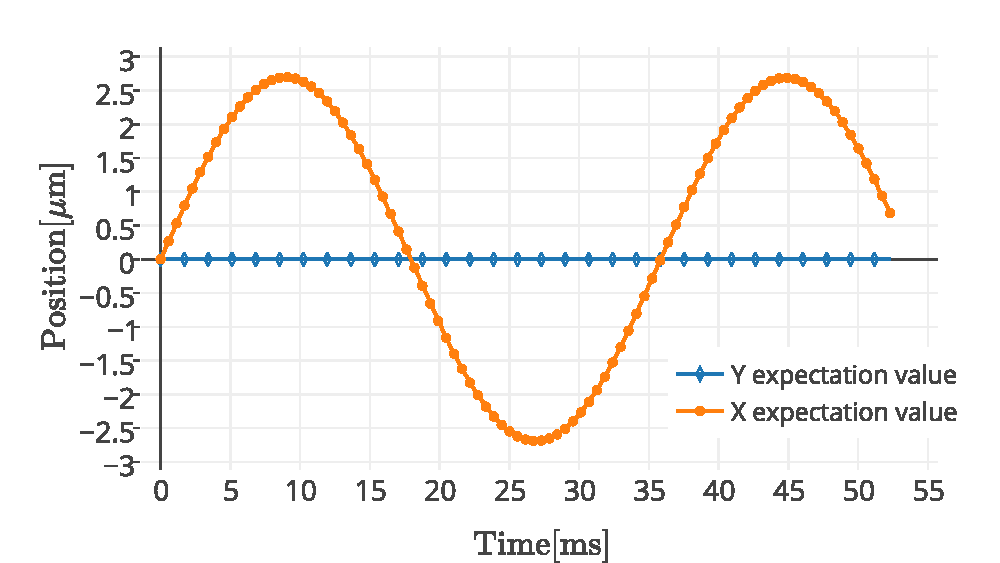
\includegraphics[width=10cm]{Plots/oscillation.pdf}
	\caption{Calculated expectation values $\braket{X}(t)$ and $\braket{Y}(t)$. The calculated oscillation frequency along the $x$ axis, $\omega_x = 2 \pi \cdot 27.9 \, \mathrm{Hz}$, is in agrement with the external potential frequency $\omega_x = 2 \pi \cdot 28 \, \mathrm{Hz}$. There is no oscillation along the $y$ axis since no impulse is imparted in this direction.} \label{plot:oscillation}
\end{figure}

To observe soliton propagation they exploited absorption imaging, measuring the BEC density distribution. Immediately after the phase imprint, they observed a positive  density disturbance travelling in the $+x$ direction, and a dark notch left behind it, which travels in the opposite direction -- this is the soliton (Fig.~\ref{plot:density_exp_1ms} to~\ref{plot:density_exp_10ms}). The positive disturbance travels with a speed higher than the soliton.

They determined the soliton speed along the $x$ axis, measuring the distance after $5 \, \mathrm{ms}$ of propagation between the notch and the position of the imprinted phase step. At that time the soliton had not travelled far from the BEC center, so this is a good estimation of the soliton speed at the center of the condensate. They obtained a mean soliton speed of  $1.8 \pm 0.4$ mm/s. This value is lower than the mean speed of sound $\nu_0 = 2.8 \pm 0.1$ mm/s, which ensures that the dark notch is a soliton and not a sound wave~\citep{DSF00}. In our simulation, we tracked the position of the soliton along the $x$ axis for $14$ ms (Fig.~\ref{plot:soliton-xposition}). We also calculated the mean speed of the notch after it had travelled for $5$ ms, obtaining a mean speed of $1.7$ mm/s, in agreement with the experimental value.
% add short-time fit
\begin{figure}[h!]
    \centering
	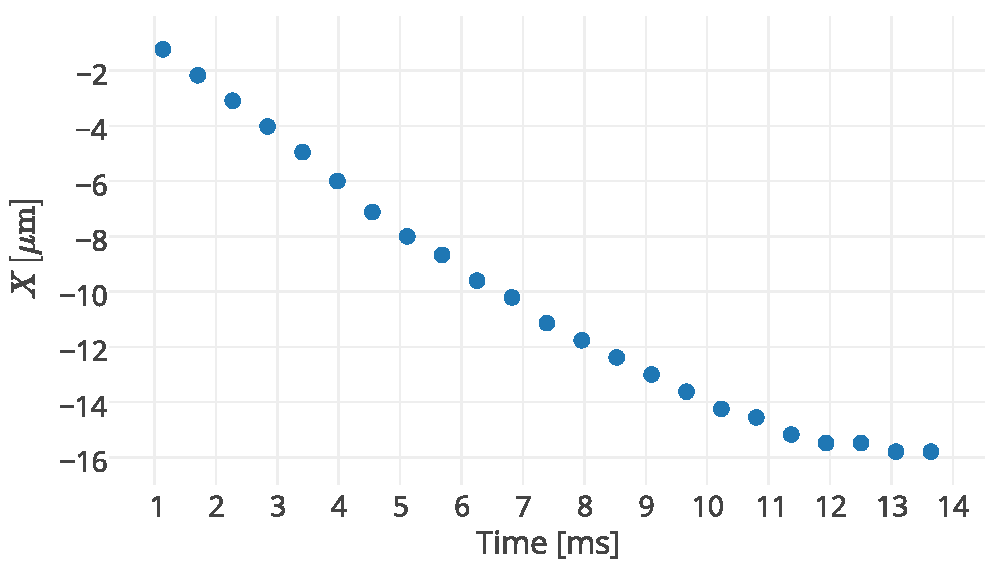
\includegraphics[width=8cm]{Plots/soliton_track.pdf}
	\caption{Calculated soliton position along the $x$ axis over the time.} \label{plot:soliton-xposition}
	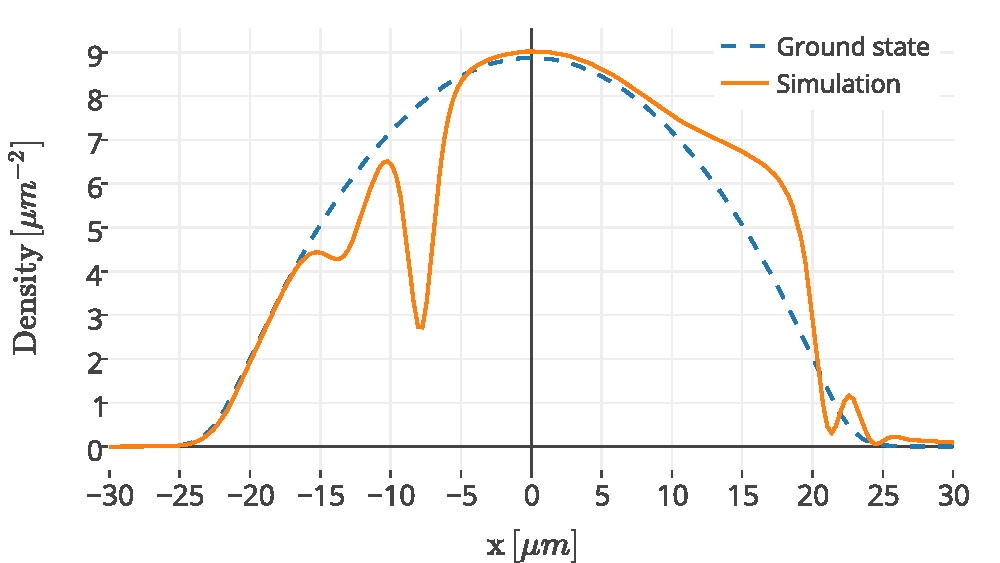
\includegraphics[width=8cm]{Plots/density_xprofile_5ms.pdf}
	\caption{Calculated ground state and particles density at $t = 5$ ms along the $x$ axis. The deep soliton is located at $x = -8 \mathrm{\mu m}$, in agreement with the experimental value~\citep{DSF00}. Other structures are visible from this figure: a shallow  dark soliton at $x = -14 \, \mathrm{\mu m}$ moving to the left; other excitations near $x = 20 \, \mathrm{\mu m}$ moving fast to the right.} \label{plot:density_5ms}
\end{figure}

The soliton speed is not the same throughout the BEC, as it depends on the particles density (Eq.~\eqref{eq:soliton-speed-density}). It is zero at the edge of the BEC, while it reaches its maximum at the center of the BEC. Indeed, rewriting Eq.~\eqref{eq:soliton-speed-density} as follows
\begin{equation}
\nu_s = \nu_0 \sqrt{1 - \frac{n - n_{min}}{n}},
\end{equation}
we see that $\nu_s$ goes to zero at the edge where both $n$ and $n - n_{min}$ go to zero, whereas the fraction $(n - n_{min}) / n$ reaches its lowest value at the center and $\nu_s$ is maximum. This implies that the soliton assumes a curved shaped, whose
% clarify what I mean with curved shape
 curvature increases as the soliton travels far from the center. This feature of the soliton is observed both in the experiment and in our simulation (Fig.~\ref{plot:density-exp-sim}). 

In Fig.~\ref{plot:density_5ms}, the particles density profile along the $x$ axis is shown after $5$ ms from the phase imprinting. The deep soliton is located at $x = -8 \mathrm{\mu m}$, in agreement with the experimental value~\citep{DSF00}. Other structures are visible from this figure: a shallow  dark soliton at $x = -14 \, \mathrm{\mu m}$ moving to the left; other excitations near $x = 20 \, \mathrm{\mu m}$ moving fast to the right. These features are not well resolved in the experimental images, but they are in agreement with the simulations in~\citep{DSF00}.
\begin{figure}
\centering
\begin{tabular}{ccccc}
\subfloat[$1$ ms]{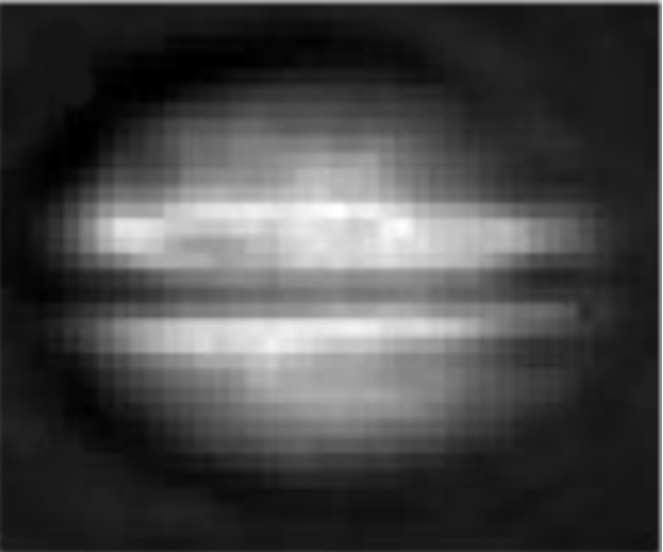
\includegraphics[width=1.9cm]{Plots/density_exp_1ms.pdf} \label{plot:density_exp_1ms}} & 
\subfloat[$2$ ms]{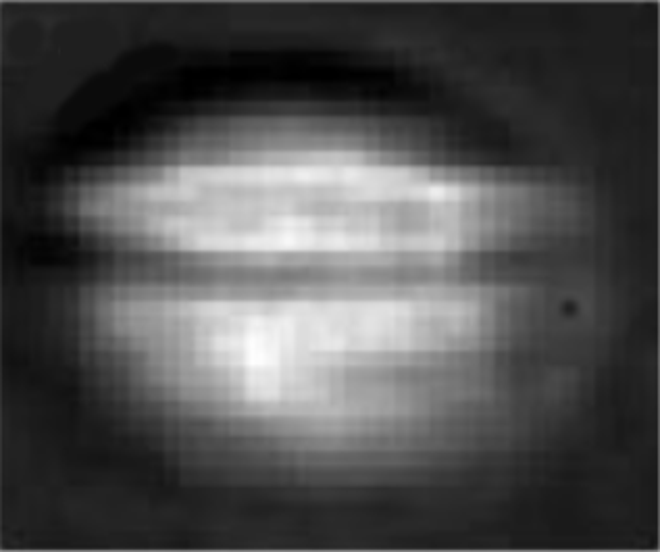
\includegraphics[width=1.9cm]{Plots/density_exp_2ms.pdf} \label{plot:density_exp_2ms}} & 
\subfloat[$5$ ms]{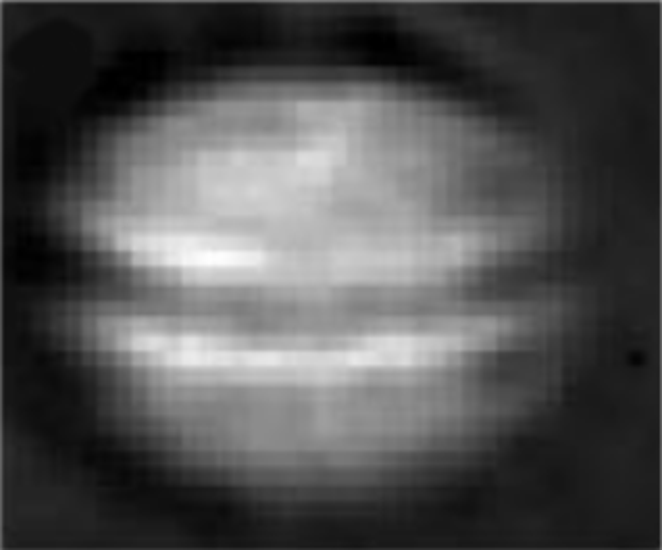
\includegraphics[width=1.9cm]{Plots/density_exp_5ms.pdf} \label{plot:density_exp_5ms}} & 
\subfloat[$7$ ms]{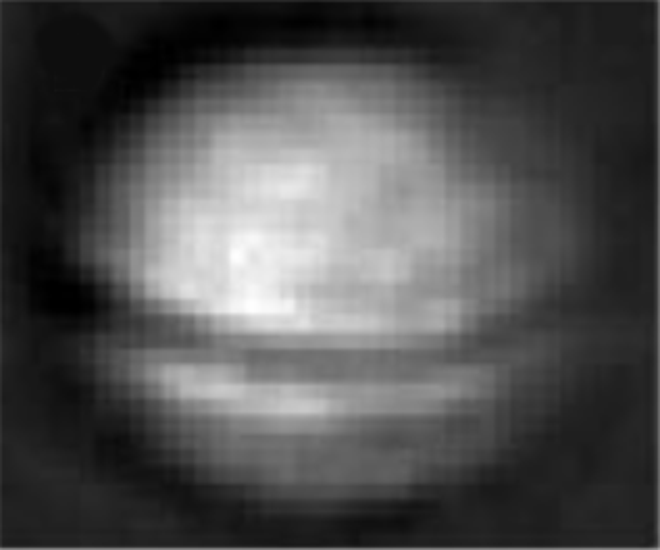
\includegraphics[width=1.9cm]{Plots/density_exp_7ms.pdf} \label{plot:density_exp_7ms}} &
\subfloat[$10$ ms]{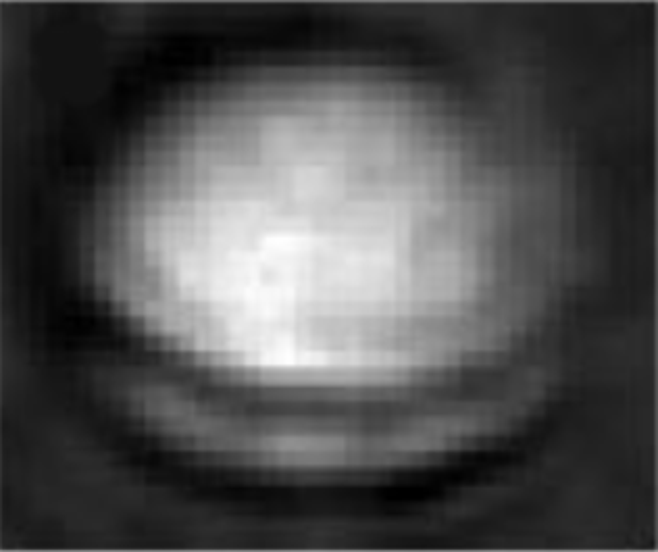
\includegraphics[width=1.9cm]{Plots/density_exp_10ms.pdf} \label{plot:density_exp_10ms}} \\
\subfloat[$1$ ms]{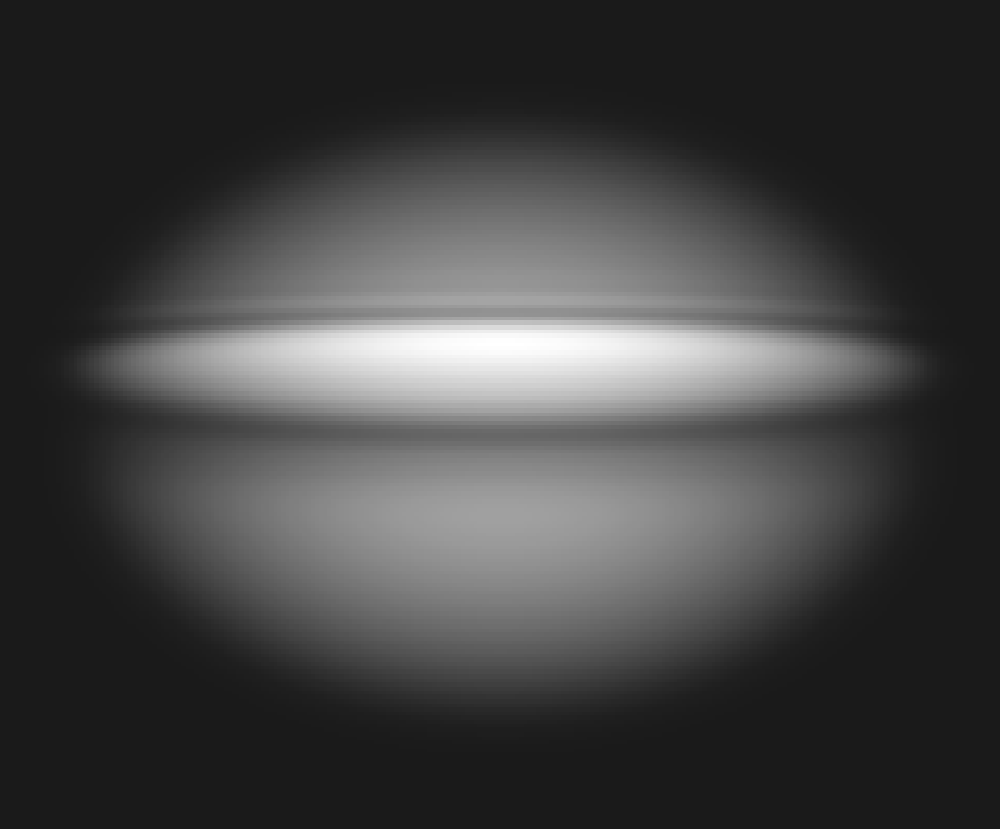
\includegraphics[width=1.9cm]{Plots/density_hmap_1ms.pdf} \label{plot:density_sim_1ms}} & 
\subfloat[$2$ ms]{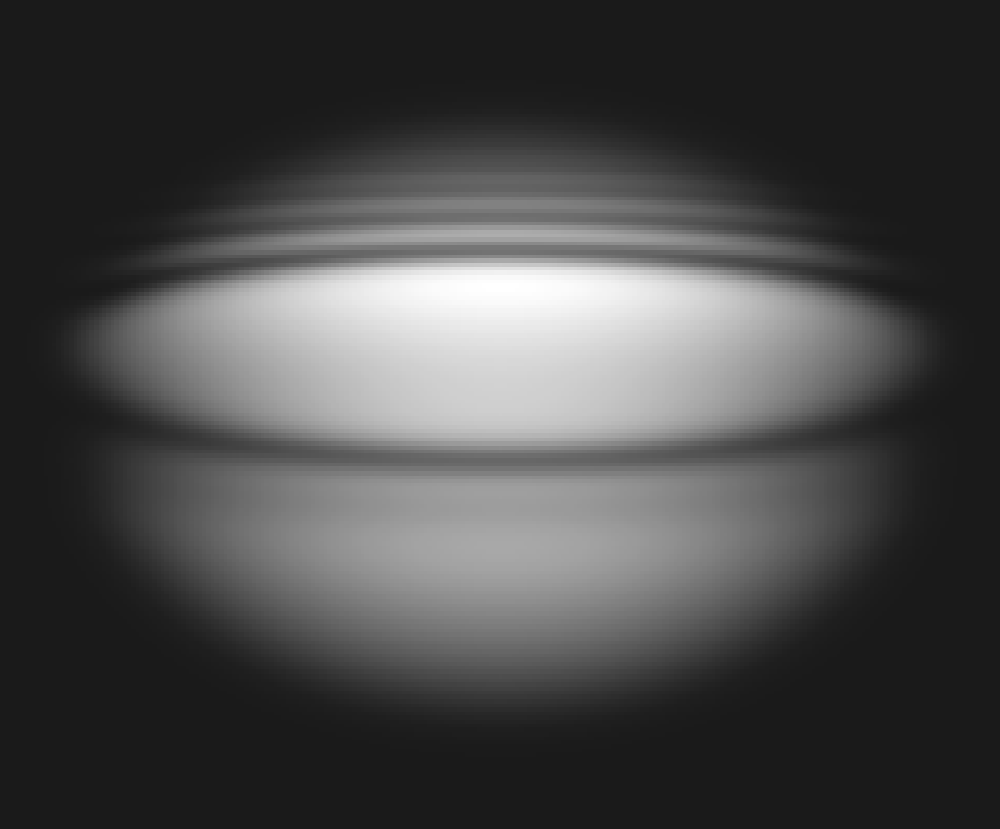
\includegraphics[width=1.9cm]{Plots/density_hmap_2ms.pdf} \label{plot:density_sim_2ms}} & 
\subfloat[$5$ ms]{
\includegraphics[width=1.9cm]{Plots/density_hmap_5ms.pdf} \label{plot:density_sim_5ms}} & 
\subfloat[$7$ ms]{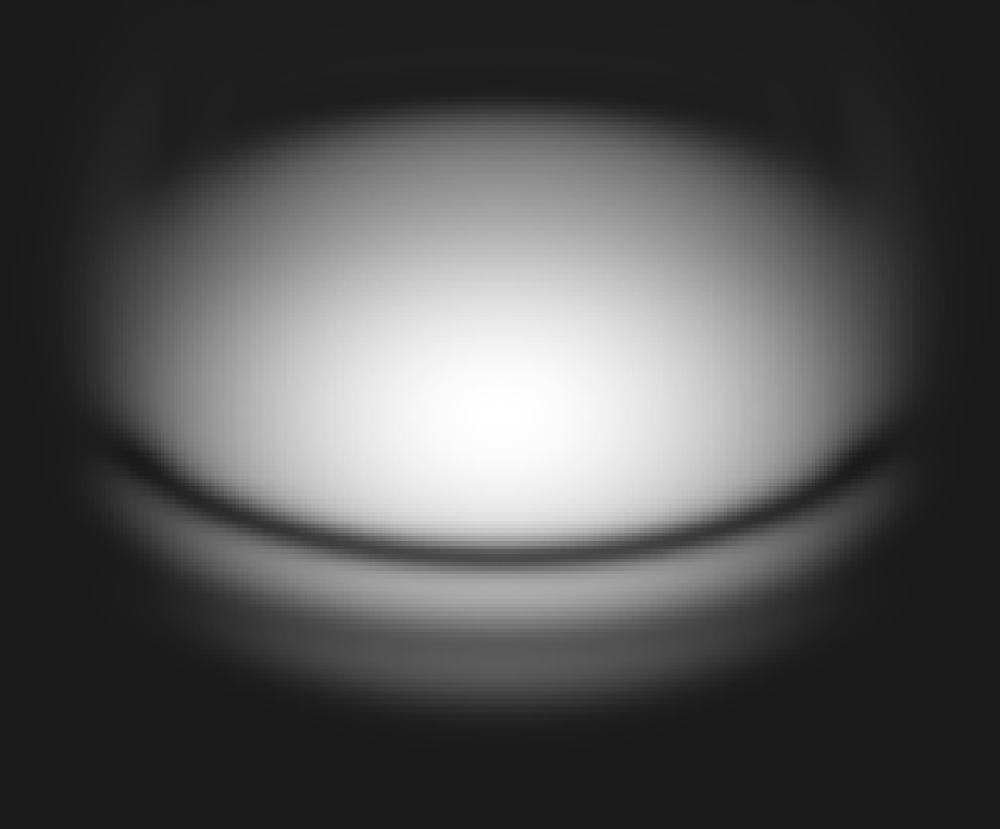
\includegraphics[width=1.9cm]{Plots/density_hmap_7ms.pdf} \label{plot:density_sim_7ms}} &
\subfloat[$10$ ms]{
\includegraphics[width=1.9cm]{Plots/density_hmap_10ms.pdf} \label{plot:density_sim_10ms}} \\
\end{tabular}
\caption{Experimental images of the integrated BEC density ((a) to (e))~\citep{DSF00} and calculated density, from our simulation, ((f) to (j)) for various times after the phase imprinting. A positive density disturbance is created and moves rapidly in the $+x$ direction. A dark soliton is left behind moving in the opposite direction at significantly less than the speed of soud.} \label{plot:density-exp-sim}
\end{figure}

Since the external potential has a minimum, the soliton is expected to oscillate with a frequency of $\omega_s = \omega_x / \sqrt{2}$. This behaviour was also found by previous simulations~\citep{MLS99,BA98}. In our case, the soliton should stop after one-quarter of the oscillation time: $T_s/4 = \frac{\pi}{\sqrt{2} \omega_x} = 12.6 \, \mathrm{ms}$, which is in good agreement with our simulation (Fig.~\ref{plot:soliton-xposition}).

We were able to evaluate a quarter of period of the soliton and not the whole period because after the notch stops it breaks up, becoming rather perturbed (Fig.~\ref{plot:density-breaksup}). This behaviour is found also in the simulations carried out in~\citep{DSF00}. 
%%%%%%%%%%%%%%%%%%%%%% EXPLAIN WHY THE SOLITON DISAPPEAR %%%%%%%%%%%%%%%
\begin{figure}[h!]
\centering
\begin{tabular}{ccccc}
\subfloat[$14$ ms]{
\includegraphics[width=2cm]{Plots/density_hmap_14ms.pdf} \label{plot:density_sim_14ms}} & 
\subfloat[$17$ ms]{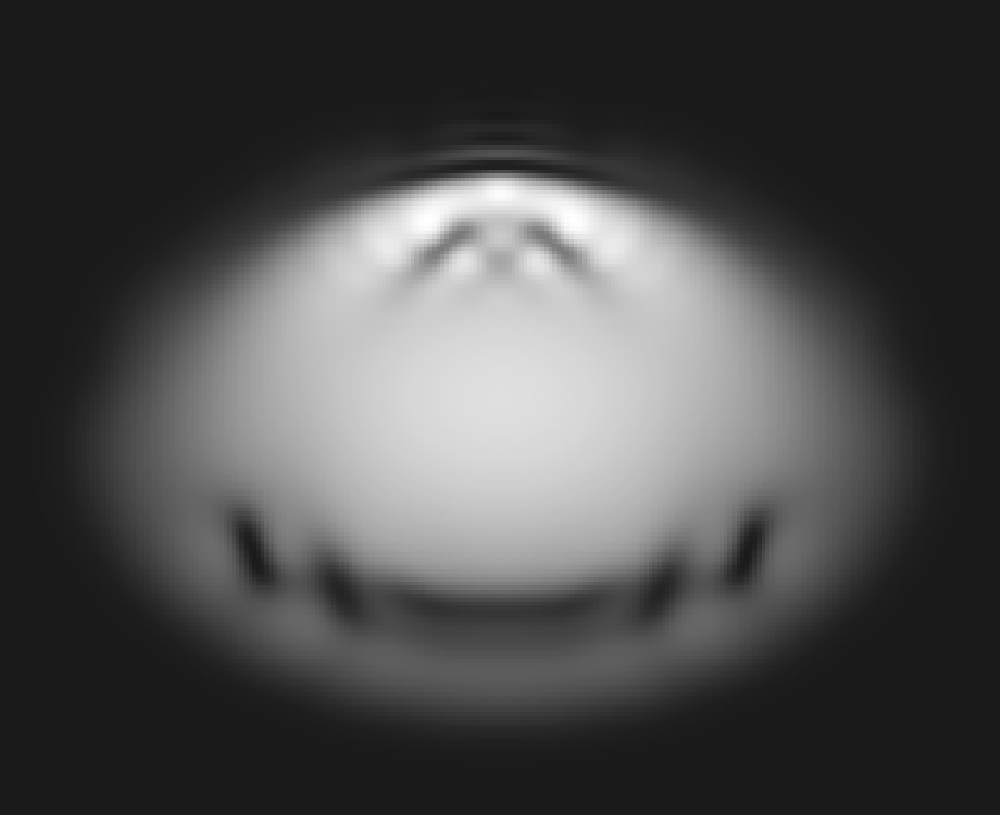
\includegraphics[width=2cm]{Plots/density_hmap_17ms.pdf} \label{plot:density_sim_17ms}} & 
\subfloat[$18$ ms]{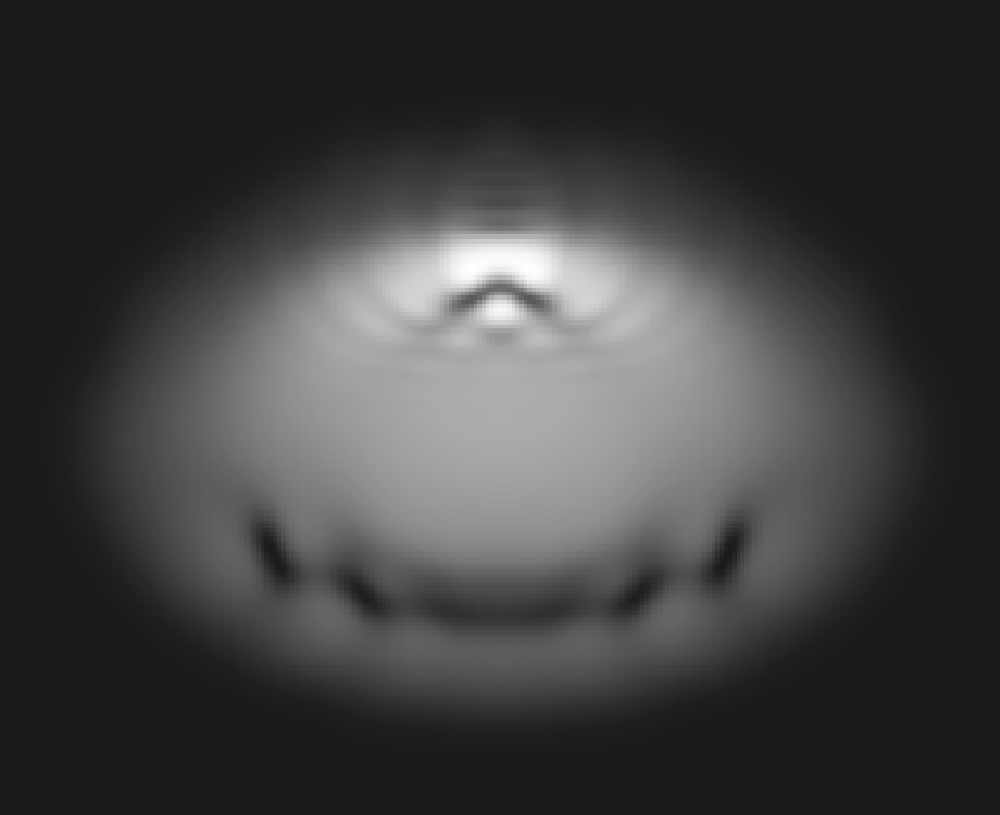
\includegraphics[width=2cm]{Plots/density_hmap_18ms.pdf} \label{plot:density_sim_18ms}} & 
\subfloat[$20$ ms]{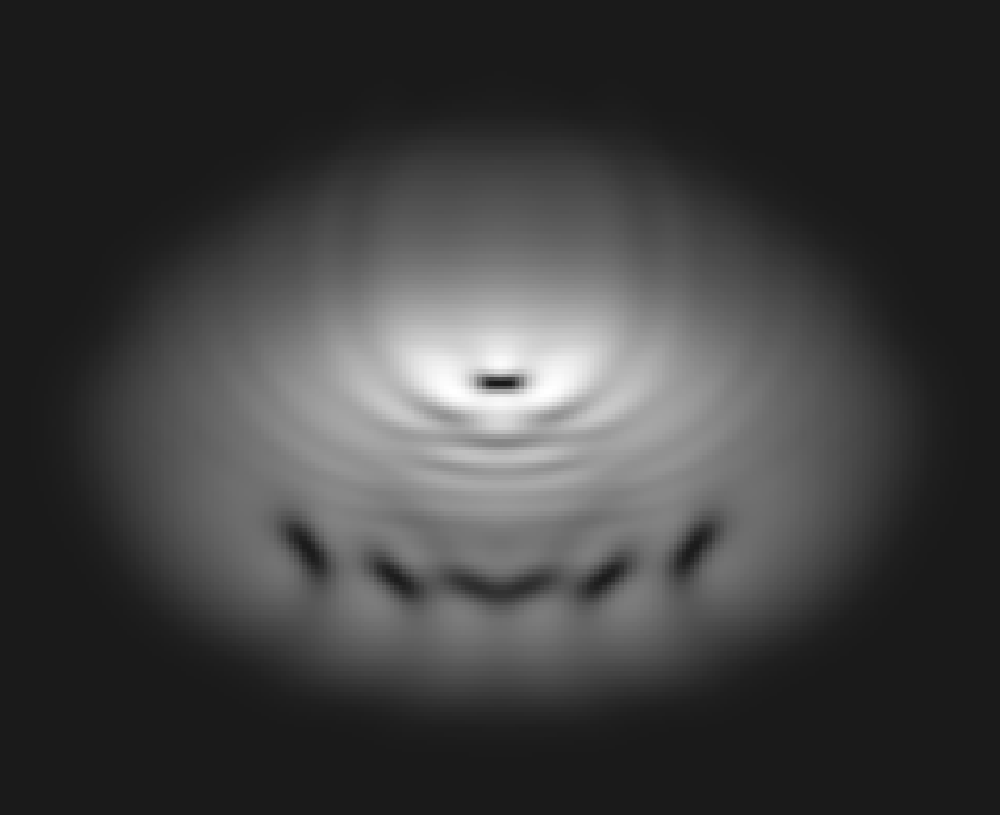
\includegraphics[width=2cm]{Plots/density_hmap_20ms.pdf} \label{plot:density_sim_20ms}} \\
\end{tabular}
\caption{Calculated particles density for various times after the soliton stops. These images show how the soliton breaks up.} \label{plot:density-breaksup}
\end{figure}